\documentclass[10pt,a4paper]{article}

\usepackage[utf8]{inputenc}
\usepackage[margin=1in]{geometry}
\thispagestyle{empty}

\usepackage{amsmath}
\usepackage{amsfonts}
\usepackage{amssymb}

\usepackage{parskip}

\usepackage{listings}
\usepackage{xcolor}

\usepackage{enumerate}

\usepackage{hyperref}

\usepackage{float}
\restylefloat{figure}
\usepackage[font=small,labelfont=bf]{caption}
\usepackage{wrapfig}

\usepackage{graphicx}
\restylefloat{figure}

\usepackage{cancel}

\usepackage{multicol}
\setlength{\columnsep}{22pt}

\usepackage{colortbl}

\author{Cristian Escudero}
\title{Redes y Comunicaciones de Datos I \\ \small{Basado en el resumen de Fede Villa}}

\begin{document}
\maketitle

\section{Conceptos Básicos}

\textit{Telemática}: ciencia que utiliza las telecomunicaciones para potenciar las posibilidades y aplicaciones de la informática.

\subsection{Arquitectura de Redes}
\begin{description}
\item \textbf{Redes de computadoras.} Conjunto de computadoras autónomas \textbf{interconectadas}.

Dos computadoras están \textit{interconectadas} cuando pueden intercambiar información, servicios, recursos, etc. Esta interconexión puede realizarse a través de distintos medios, como ser \textit{cables de cobre, fibra óptica, microondas, rayos infrarrojos, satélites, etc}. 

\item \textbf{Sistemas distribuidos.} Un conjunto de computadoras independientes aparece ante sus usuarios como un sistema consistente y único.
\end{description}
La diferencia entre ambas está en el \textbf{software} (en el SO sobretodo), más que en el \textbf{hardware}.

\subsection{Dispositivos utilizados para la interconexión de Redes}

\begin{itemize}
\item \textit{Repetidores} (regeneran la señal) y \textit{amplificadores} (la amplifican).
\item \textit{Puentes} (Bridges).
\item \textit{Conmutador o Router}: Dispositivo especializado en la conmutación de paquetes. Generalmente utiliza un hardware y software diseñados a propósito.
\item \textit{Gateway}.
\end{itemize}

\subsection{Clasificación de las Redes}
\subsubsection{Según tecnología de transmisión}
\begin{description}
\item \textbf{Enlaces de difusión} (\textit{redes broadcast).} Estas redes tienen un solo canal de comunicación por lo que todas las máquinas de la red lo comparten; si una máquina envía un \textbf{paquete}, todas las demás lo reciben. Cuando las máquinas reciben un paquete verifican la dirección de destino (guardada dentro del paquete) y solo el destinatario lo procesara, los demás lo desecharán. ``\textit{La información se envía a todos los nodos de la red, aunque solo interese a unos pocos}''.

Estos sistemas soportan también el envío de paquetes con una dirección de difusión (\textit{broadcast}) en el destinatario, en este caso todos los que reciben el paquete lo procesaran. Por último puede enviarse un paquete a un conjunto de máquinas, esto se conoce como multidifusión (\textit{multicasting}).

Se pueden crear \textbf{redes planas}, es decir redes en las que la comunicación entre dos ordenadores cualesquiera se haga de forma directa, sin routers intermedios. Presenta posibles problemas de seguridad.

\item \textbf{Enlaces punto a punto.} Estas redes constan de muchas conexiones entre pares individuales de máquinas. Para ir del origen al destino, un paquete en este tipo de red podría tener que visitar primero a una o varias máquinas intermedias. El transporte de datos en estas redes se conoce como unidifusión (\textit{unicasting}). ``\textit{La información se envía solo al nodo al cual va dirigida}''.

Generalmente la comunicación entre dos ordenadores cualesquiera se realiza a través de nodos intermedios que \textbf{encaminan} o \textbf{conmutan} los paquetes. En un enlace punto a punto, el conjunto de router o conmutadores y los enlaces que los unen forman lo que se conoce como \textbf{subred}.

Además, permite crear topologías complejas (\textit{anillo, malla, estrella, etc}).
\end{description}
\textit{Nota:} Las redes de poca cobertura geográfica tienden a utilizar la \textit{difusión}, mientras que las de cobertura más grande usan la \textit{punto a punto}.

\begin{wrapfigure}{r}{0.5\textwidth}
  \caption{Topologías LAN típicas, izquierda \textbf{bus} (\textit{ethernet}) y derecha \textbf{anillo} (\textit{token ring}).}
  \label{fig:topologia_lan}  
  \centering
  \hbox{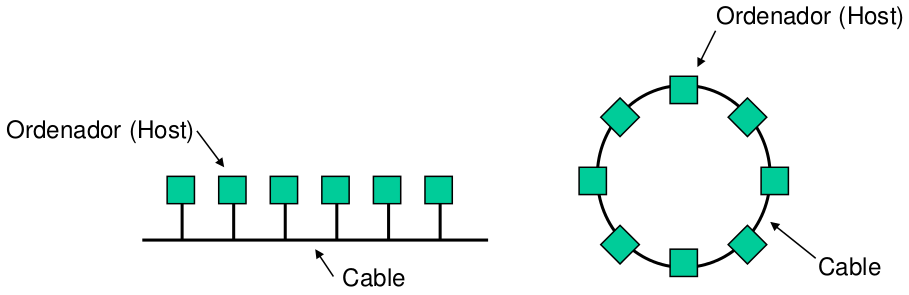
\includegraphics[width=0.5\textwidth-\fboxrule-\fboxrule]{imgs/topologia_lan.png}}  
\end{wrapfigure}

\begin{wrapfigure}{r}{0.5\textwidth}
  \caption{Escenario típico de una red completa.}
  \label{fig:escenario_lan_wan}  
  \centering
  \hbox{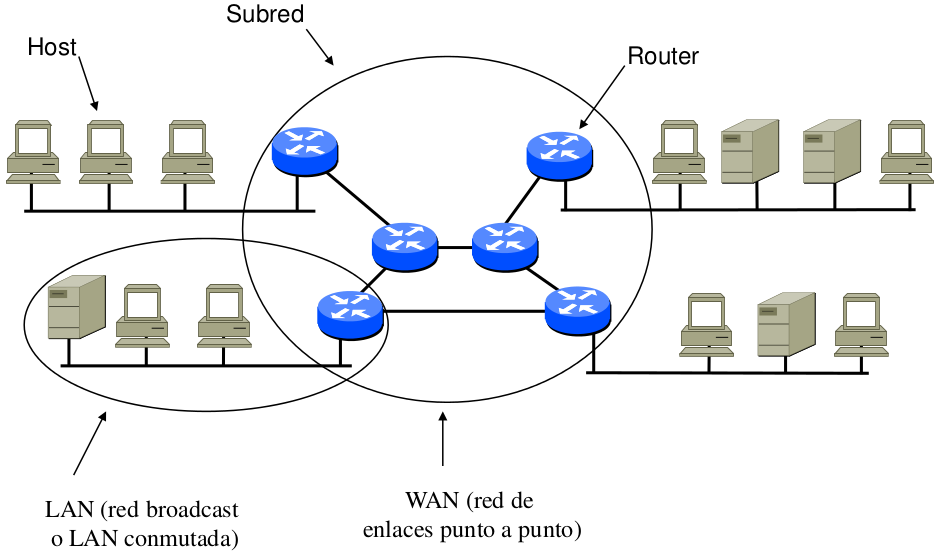
\includegraphics[width=0.5\textwidth-\fboxrule-\fboxrule]{imgs/escenario_lan_wan.png}}  
\end{wrapfigure}

\subsubsection{Según su cobertura geográfica}

\begin{description}
\item \textbf{PAN} (\textit{$\approx 1$ metro}). Destinadas a una sóla persona.

\textit{Ejemplo}: una red que conecta los distintos dispositivos de una computadora.
\item \textbf{LAN} (\textit{$\leq 1$ km}). Redes privadas cuyo ámbito no sobrepasa un edificio o campus. Se caracterizan por su alcance, tecnología de transmisión (generalmente \textit{broadcast}), y topología. Están diseñadas desde el principio para transportar datos. El cableado es propiedad del usuario normalmente.

\textit{Ejemplos}: ethernet, token ring, redes inalámbricas por radio.

\item \textbf{MAN} ($\leq 10$ \textit{km}). Abarca una ciudad.

\textit{Ejemplo:} Red de televisión por cable disponible en muchas ciudades.

\item \textbf{WAN} ($\leq 1000$ \textit{km}). Tienen velocidades de transferencia de datos menores a las LANs. Utilizan la base del sistema telefónico, diseñado inicialmente para transportar voz. Son servicios contratados generalmente a operadoras. Suelen utilizar enlaces \textbf{punto a punto} \textit{temporales} o \textit{permanentes}, salvo las comunicaciones vía satélite que son \textit{broadcast}. Tienen un costo elevado, por lo que se suele optimizar su diseño.
\end{description}

\section{Software de Redes}

La interconexión de computadoras es un problema técnico de complejidad elevada y la mejor forma de resolver un problema complejo es dividirlo en partes. En telemática dichas partes se llaman \textbf{capas}, que tienen funciones bien definidas, y están construidas una encima de la otra. El propósito de cada capa es ofrecer ciertos servicios a las capas superiores, a las cuales no se le muestran los detalles de implementación de los servicios ofrecidos.

\subsection{Modelo de Capas}
Actualmente todas las \textit{arquitecturas de red} se describen utilizando un \textbf{modelo de capas}, que permite describir el funcionamiento de las redes de forma modular y hacer cambios de manera sencilla.

\subsubsection{Conceptos básicos}
\begin{description}
\item \textbf{Servicio.} Conjunto de primitivas (\textbf{operaciones}) que una capa proporciona a la capa que está sobre ella. Esta define que operaciones puede realizar la capa en beneficio de sus usuarios, pero no dice nada respecto a su implementación. Se relacionan con las interacciones entre capas.
\item \textbf{Protocolo.} Conjunto de reglas que rigen el formato y significado de los paquetes que intercambian las entidades iguales en una capa. Se relacionan con los paquetes enviados entre entidades iguales de máquinas diferentes.
\item \textbf{Interfaz.} Define que operaciones y servicios primitivos pone la capa más baja a disposición de la capa superior inmediata. Si están bien definidas, simplifican el reemplazo de la implementación de una capa por otra implementación totalmente diferente, siempre que se mantengan exactamente los mismos servicios ofrecidos a la capa superior en ambas implementaciones.
\end{description}

Los datos no se transfieren de manera directa de la capa $n$ de una máquina a la capa $n$ de la otra máquina, sino que cada capa pasa los datos y la información de control a la capa inmediatamente inferior, hasta alcanzar la capa más bajo. Debajo de la \textit{capa 1} se encuentra el \textbf{medio físico} a través del cual ocurre la comunicación real.

Un conjunto de capas y protocolos se conoce como \textbf{arquitectura de red}. Ni los detalles de la implementación ni las especificaciones de las interfaces son parte de esta, ya que están ocultas en el interior de la máquina. La lista de protocolos utilizados por un sistema, un protocolo por capa, se conoce como \textbf{pila de protocolos}.

\subsubsection{Objetivos Fundamentales}
\begin{itemize}
\item \textbf{Sencillez}: Hace abordable el complejo problema de la comunicación entre ordenadores.
\item \textbf{Modularidad}: Permite realizar cambios relativamente fáciles a alguna de sus partes sin afectar al resto.
\item \textbf{Compatibilidad}: La comunicación entre dos entidades de una capa puede realizarse independientemente de las demás.
\end{itemize}

\subsubsection{Principios}
\begin{itemize}
\item La capa $n$ ofrece sus servicios a la capa $n+1$.
\item La capa $n+1$ solo usa los servicios de la capa $n$.
\item La capa $n$ solo habla con la capa $n$ de otro sistema (\textit{peer to peer}, ó comunicación igual a igual) siguiendo el protocolo de la capa $n$.
\end{itemize}

\subsubsection{Servicios Orientados a la Conexión y No Orientados a la Conexión}

Las capas pueden ofrecer estos dos tipos de servicios a las capas que están sobre ellas.
\begin{description}
\item \textbf{Orientado a Conexión.} Se concibió en base al sistema telefónico: el usuario del servicio primero establece una conexión, la utiliza, y luego la abandona.

\textit{Características:} Se respeta el orden de los paquetes. Se mantiene la misma ruta o camino para todos los paquetes. Si el canal se corta la comunicación se interrumpe.
\item \textbf{No Orientado a Conexión.} Se concibió en base al sistema postal: cada mensaje lleva completa la dirección de destino y cada uno se enruta a través del sistema, independientemente de los demás.

\textit{Características:} No se respeta el orden de los paquetes. La ruta puede variar para cada paquete. La red es más robusta ya que si una ruta queda inservible, pueden usarse otras. Si la comunicación  no es posible los datos se pierden.
\end{description}

\subsection{Modelo OSI}

\subsubsection{Principios}
\begin{itemize}
\item Una capa se debe crear donde se necesite una abstracción bien definida.
\item Cada capa debe realizar una función bien definida.
\item La función de cada capa se debe elegir con la intención de definir protocolos estandarizados internacionalmente.
\item Los limites de las capas se deben elegir a fin de minimizar el flujo de información a través de las interfaces.
\item La cantidad de capas debe ser suficientemente grande para no tener que agrupar funciones distintas en la misma capa y lo bastante pequeña para que la arquitectura no se vuelva inmanejable.
\end{itemize}

\subsubsection{Capas del OSI}
\begin{description}
\item \textbf{Aplicación:} Capa que acoge a todas las aplicaciones que requieren la red. Es la interfaz que ve el usuario. Envía los datos de usuario a la aplicación de destino usando servicios de las capas inferiores.
\item \textbf{Presentación:} Encargada de la sintaxis de los datos. Convierte los datos de la red a los datos requeridos por la aplicación.
\item \textbf{Sesión:} Encargada de proporcionar dialogo para el uso eficiente de las comunicaciones. O sea, sincroniza el intercambio de datos entre capas inferiores y superiores.
\item \textbf{Transporte:} Esta capa se encarga de que los datos enviados y recibidos lleguen en orden, sin duplicar y sin errores. Puede ser orientado o no a la conexión.
\item \textbf{Red:} Se encarga de enlazar con la red y encaminar los datos hacia sus lugares o direcciones de destino. Brinda la información de hacia dónde debo ir. Esta y las dos capas inferiores se encargan de todo el proceso externo al propio sistema y que están tanto en terminales como en enlaces o repetidores.
\item \textbf{Enlace de datos:} Se encarga de que los datos se envíen con seguridad a su destino y libre de errores. Cuando la conexión no es punto a punto, esta capa no puede asegurar su cometido sino la capa superior. Tiene el control de la capa física.
\item \textbf{Física:} Transmite los datos y suministra servicios a la siguiente capa. Para ello debe conocer las características mecánicas, eléctricas, funcionales y de procedimiento de las líneas.
\end{description}

\subsection{Modelo TCP/IP e Híbrido}

Los protocolos \textbf{TCP/IP} nacieron por la necesidad de ínter-operar redes diversas (\textit{inter-networking}). Se diseño después de los protocolos, por eso a diferencia del \textit{modelo OSI} este tiene protocolos ``predefinidos''. No funciona con otra pila de protocolos.

Cuando se usa un modelo siguiendo el OSI en las capas bajas y el TCP/IP en las altas, se dice que se utiliza un modelo \textbf{híbrido}.

La descomposición del problema de la comunicación en capas es similar que en el OSI. El problema de OSI es que en una capa, todos los protocolos deben tener un funcionamiento similar además de utilizar las funciones definidas en la capa inferior y de suministrar funciones a la capa superior.

\begin{wrapfigure}{r}{0.7\textwidth}
  \caption{Comparación de los distintos modelos.}
  \label{fig:comparacion_modelos}  
  \centering
  \hbox{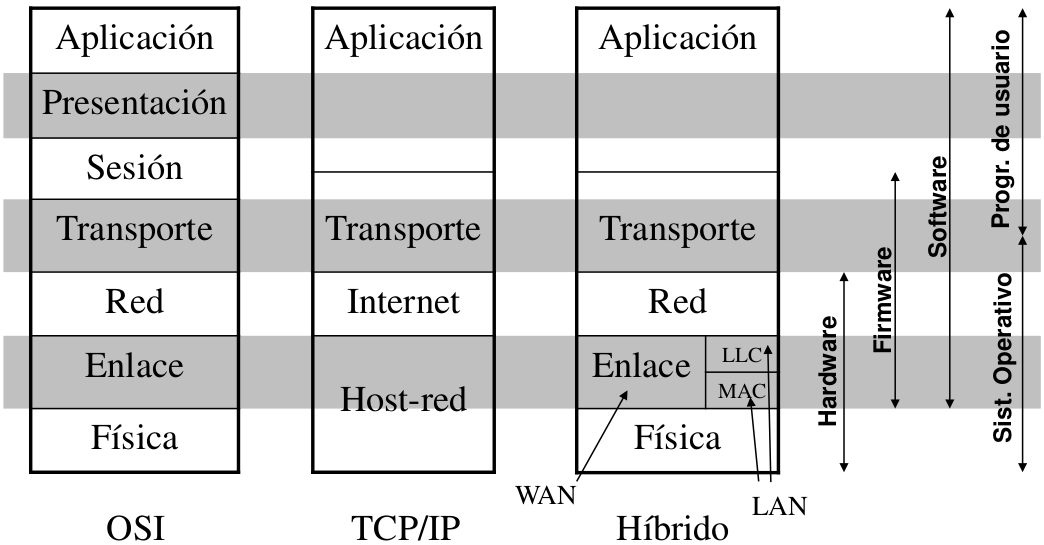
\includegraphics[width=0.7\textwidth-\fboxrule-\fboxrule]{imgs/comparacion_modelos.png}}  
\end{wrapfigure}

\subsubsection{Capas de TCP/IP}
\begin{description}
\item \textbf{Aplicación:} Proporciona comunicación entre procesos o aplicaciones en computadores distintos.
\item \textbf{Transporte:} Encargada de transferir datos ente computadores sin detalles de red pero con mecanismos de seguridad.
\item \textbf{Interred:} Se encarga de direccionar y guiar los datos desde el origen al destino a través de la red o redes intermedias.
\item \textbf{Enlace de datos:} Interfaz entre el sistema final y la \textit{subred} a la que está conectado.
\item \textbf{Física:} Define las características del medio, señalización y codificación se las señales.
\end{description}

\begin{wrapfigure}{r}{0.5\textwidth}
  \caption{Protocolos y redes del modelo TCP/IP inicial.}
  \label{fig:tcp_ip}  
  \centering
  \hbox{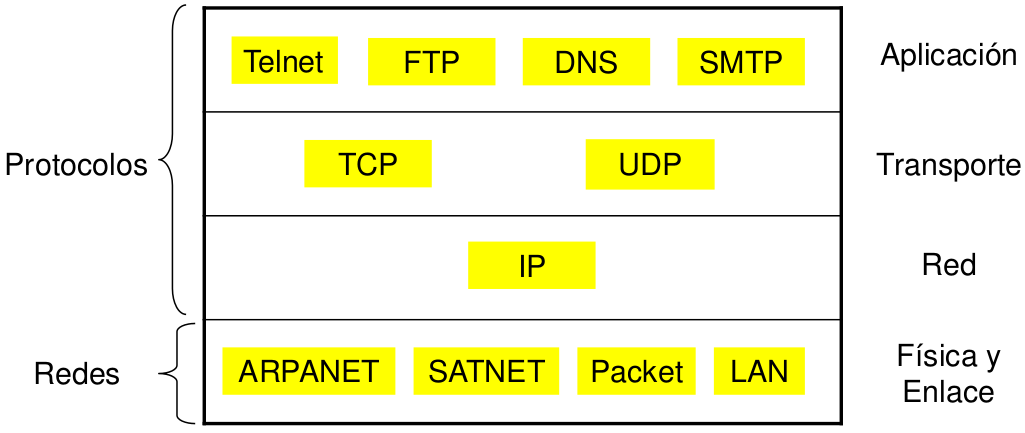
\includegraphics[width=0.5\textwidth-\fboxrule-\fboxrule]{imgs/tcp_ip.png}}  
\end{wrapfigure}

\subsubsection{Diferencias entre OSI y TCP/IP}
\begin{itemize}
\item En OSI primero fue el modelo, después los protocolos. En TCP primero los protocolos, después el modelo.
\item En OSI el modelo es bueno, los protocolos malos; en TCP/IP al revés.
\item En OSI los productos llegaban tarde, eran caros y tenían muchas fallas; en TCP/IP todo lo contrario.
\item En TCP/IP los productos aparecían rápido, estaban muy probados (pues los usaba mucha gente), y a menudo eran gratis.
\item OSI soporta comunicación orientada y no orientada a la conexión en la capa de red, pero solo orientada en la capa de transporte; TCP/IP usa un modo no orientado en la capa de red y ambos en la capa de transporte.
\end{itemize}

\subsubsection{OSI modificado}
El que vamos a utilizar. Sus capas son:
\begin{itemize}
\item \textbf{Aplicación} (incluye \textit{sesión} y \textit{presentación}).
\item \textbf{Transporte.}
\item \textbf{Red.}
\item \textbf{Enlace de datos.}
\subitem + Subcapa LLC (\textit{Logical Link Control}).
\subitem + Subcapa MAC (\textit{Media Access Control}).
\item \textbf{Física.}
\end{itemize}

\end{document}